\section{Mallin testaus}
Tässä osiossa esitellään esimerkit fantomien sädepohjaisesta SPECT-rekonstruktiosta jokaisella kolmella mallilla. Rekonstruktiota verrataan olemassa olevaan kuva-alueen rotaatioon perustuvaan rekonstruktioon, jonka lisäksi tarkastellaan säteiden määrän vaikutusta rekonstruktion laatuun ja laskentanopeuteen. Rekonstruktiot yhteensä neljällä eri projektiomenetelmällä ovat esitetty kuvissa \ref{fig:nema-rekonstruktiot}, \ref{fig:cbf-rekonstruktiot} ja \ref{fig:rekonstruktiot}. Jokaisen rekonstruktion arvot ovat skaalattu välille [0, 1] siten, että pienin arvo vastaa lukua 0 ja suurin lukua 1. Kuvien värikartoissa 0 vastaa mustaa ja 1 valkoista väriä. Rekonstruktioissa käytettiin OSEM-algoritmia kahdella iteraatiolla ja 8 osajoukolla. Kuva-alueen koko oli $128^3$ vokselia ja gammakameran parametrit kuten simulaatioissa ja mittauksissa. Laskennassa käytetty suoritin oli Intel i7-10850H.

Keskusyksiköllä laskenta on verrattain hidasta ja esimerkiksi 144 säteellä laskenta kestää noin viisi minuuttia. Tästä syystä SPECT-rekonstruktion validoinnissa käytettiin mallia 3, jolla rekonstruktio onnistuu jo 1 säteellä. Esimerkiksi mallissa 1 säteiden minimimäärä on detektorin pikselin päälle asettuvien kollimaattorin reikien lukumäärä, eli useita kymmeniä. Mallia 3 testattiin suorittamalla NEMA-fantomin simuloidun projektiodatan rekonstruktio eri säteiden lukumäärällä 100 kertaa, jotta laskenta-ajan vaihtelu olisi mahdollista määrittää. Vaihtelua laskenta-ajassa luovat pääosin käyttöjärjestelmän muut taustalla suoritettavat prosessit sekä tietokoneen korkeasta lämpötilasta johtuva laskentatehon väheneminen.

\begin{figure}[H]
    \centering
    \captionsetup{width=.9\linewidth}
    \begin{subfigure}[t]{.25\textwidth}
        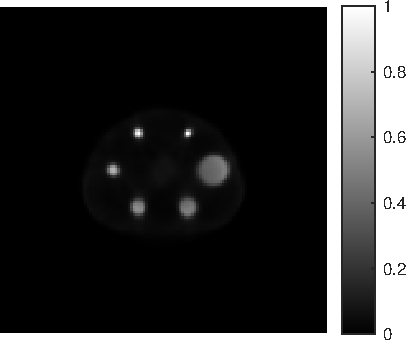
\includegraphics[width=\linewidth]{kuvat/nema_rekonstruktio_proj6.pdf}
        \caption{Kuva-alueen rotaatioon perustuva projektiomenetelmä}
    \end{subfigure}%
    \hspace{.075\textwidth}%
    \begin{subfigure}[t]{.25\textwidth}
        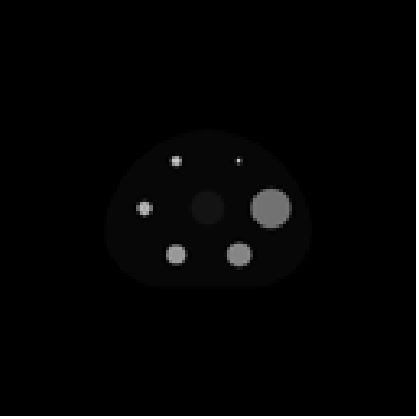
\includegraphics[width=\linewidth]{kuvat/nema_ground_truth.pdf}
        \caption{Todellinen aktiivisuusjakauma}
    \end{subfigure}%
    \hspace{.075\textwidth}%
    \begin{subfigure}[t]{.25\textwidth}
        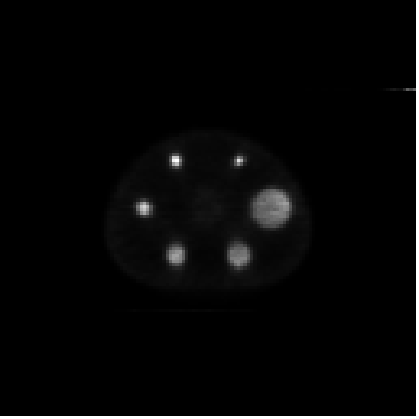
\includegraphics[width=\linewidth]{kuvat/nema_rekonstruktio_proj1_malli1_nRay7.pdf}
        \caption{Sädepohjainen projektiomenetelmä, malli 1, 7 sädettä}
    \end{subfigure}
    \begin{subfigure}[b]{.25\textwidth}
        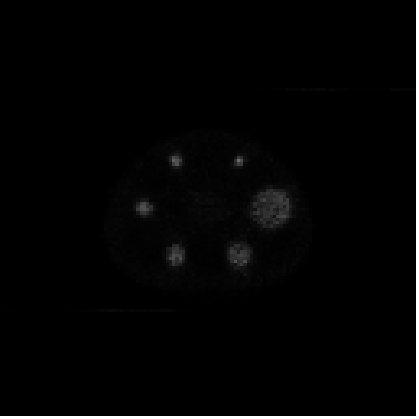
\includegraphics[width=\linewidth]{kuvat/nema_rekonstruktio_proj1_malli2_nRay7.pdf}
        \caption{Sädepohjainen projektiomenetelmä, malli 2, 7 sädettä}
    \end{subfigure}%
    \hspace{.075\textwidth}%
    \begin{subfigure}[b]{.25\textwidth}
        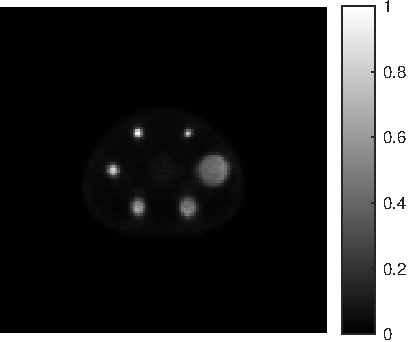
\includegraphics[width=\linewidth]{kuvat/nema_rekonstruktio_proj1_malli3_nRay9.pdf}
        \caption{Sädepohjainen projektiomenetelmä, malli 3, 9 sädettä}
    \end{subfigure}
    \caption{Simuloidun IQ NEMA -fantomin SPECT-projektiodatan rekonstruktio neljällä eri projektiomenetelmällä ja todellinen aktiivisuusjakauma. Kuvissa on esitetty poikkileikkaus kuva-alueen aktiivisuusjakaumasta. Kuvien värikartat ovat skaalattu siten, että kuva-alueen suurin arvo vastaa valkoista väriä ja kuva-alueen pienin arvo mustaa väriä. Kuvan \textbf{(c)} rekonstruktion projektiossa käytettiin 7 sädettä yhtä kollimaattorin reikää kohti. Kuvan \textbf{(e)} rekonstruktiossa säteiden määrä voi olla vain jonkin luonnollisen luvun neliö, josta johtuen rekonstruktioon valittiin 9 sädettä.}
    \label{fig:nema-rekonstruktiot}
\end{figure}

\begin{figure}[H]
    \centering
    \captionsetup{width=.9\linewidth}
    \begin{subfigure}[t]{.25\textwidth}
        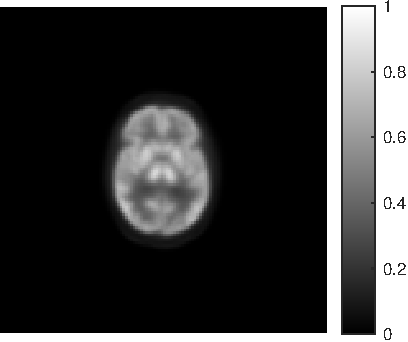
\includegraphics[width=\linewidth]{kuvat/cbf_rekonstruktio_proj6.pdf}
        \caption{Kuva-alueen rotaatioon perustuva projektiomenetelmä}
    \end{subfigure}%
    \hspace{.075\textwidth}%
    \begin{subfigure}[t]{.25\textwidth}
        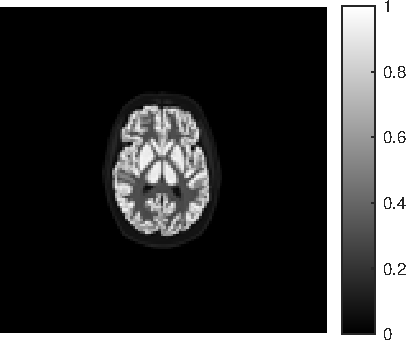
\includegraphics[width=\linewidth]{kuvat/cbf_ground_truth.pdf}
        \caption{Todellinen aktiivisuusjakauma}
    \end{subfigure}%
    \hspace{.075\textwidth}%
    \begin{subfigure}[t]{.25\textwidth}
        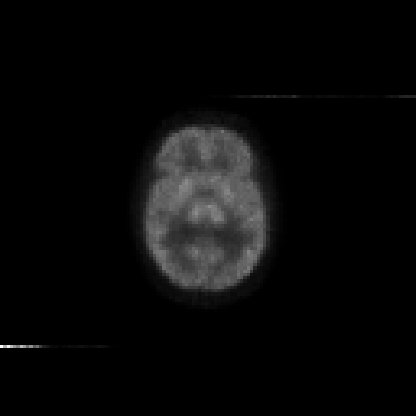
\includegraphics[width=\linewidth]{kuvat/cbf_rekonstruktio_proj1_malli1_nRay7.pdf}
        \caption{Sädepohjainen projektiomenetelmä, malli 1, 7 sädettä}
    \end{subfigure}
    \begin{subfigure}[b]{.25\textwidth}
        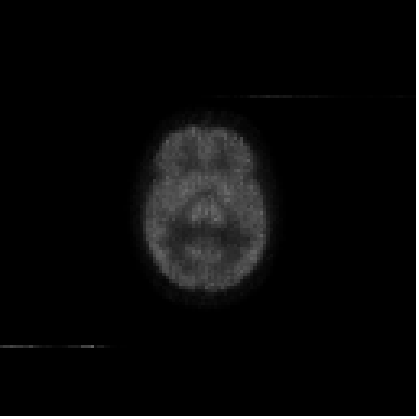
\includegraphics[width=\linewidth]{kuvat/cbf_rekonstruktio_proj1_malli2_nRay7.pdf}
        \caption{Sädepohjainen projektiomenetelmä, malli 2, 7 sädettä}
    \end{subfigure}%
    \hspace{.075\textwidth}%
    \begin{subfigure}[b]{.25\textwidth}
        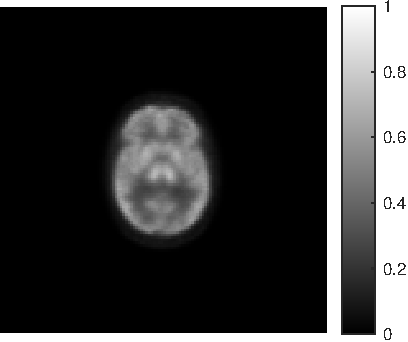
\includegraphics[width=\linewidth]{kuvat/cbf_rekonstruktio_proj1_malli3_nRay9.pdf}
        \caption{Sädepohjainen projektiomenetelmä, malli 3, 9 sädettä}
    \end{subfigure}
    \caption{Simuloidun Zubal-fantomin SPECT-projektiodatan rekonstruktio neljällä eri projektiomenetelmällä ja todellinen aktiivisuusjakauma. Kuvissa on esitetty poikkileikkaus kuva-alueen aktiivisuusjakaumasta. Kuvien värikartat ovat skaalattu siten, että kuva-alueen suurin arvo vastaa valkoista väriä ja kuva-alueen pienin arvo mustaa väriä. Kuvan \textbf{(c)} rekonstruktion projektiossa käytettiin 7 sädettä yhtä kollimaattorin reikää kohti. Kuvan \textbf{(e)} rekonstruktiossa säteiden määrä voi olla vain jonkin luonnollisen luvun neliö, josta johtuen rekonstruktioon valittiin 9 sädettä.}
    \label{fig:cbf-rekonstruktiot}
\end{figure}

\begin{figure}[H]
    \centering
    \captionsetup{width=.9\linewidth}
    \begin{subfigure}[t]{.25\textwidth}
        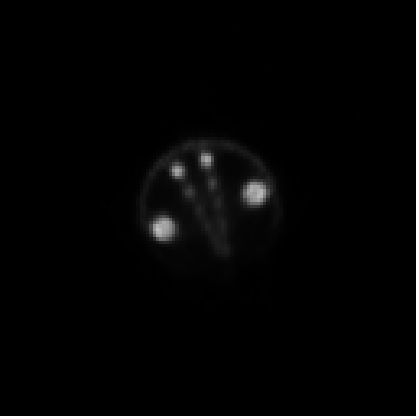
\includegraphics[width=\linewidth]{kuvat/pro_specta_rekonstruktio_proj6.pdf}
        \caption{Kuva-alueen rotaatioon perustuva projektiomenetelmä}
    \end{subfigure}%
    \hspace{.075\textwidth}%
    \begin{subfigure}[t]{.25\textwidth}
        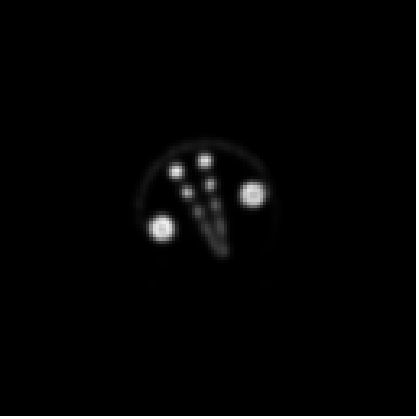
\includegraphics[width=\linewidth]{kuvat/pro_specta_ground_truth.pdf}
        \caption{Laitevalmistajan ohjelmistolla tuotettu rekonstruktio}
    \end{subfigure}%
    \hspace{.075\textwidth}%
    \begin{subfigure}[t]{.25\textwidth}
        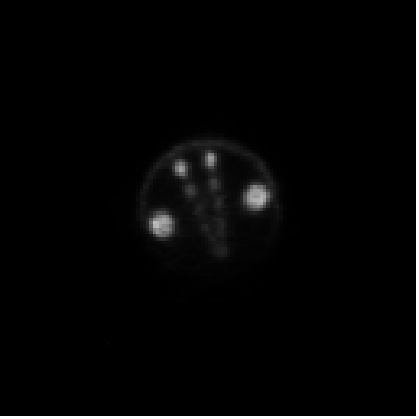
\includegraphics[width=\linewidth]{kuvat/pro_specta_rekonstruktio_proj1_malli1_nRay7.pdf}
        \caption{Sädepohjainen projektiomenetelmä, malli 1, 7 sädettä}
    \end{subfigure}
    \begin{subfigure}[b]{.25\textwidth}
        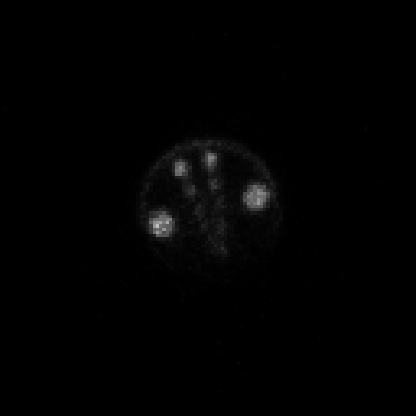
\includegraphics[width=\linewidth]{kuvat/pro_specta_rekonstruktio_proj1_malli2_nRay7.pdf}
        \caption{Sädepohjainen projektiomenetelmä, malli 2, 7 sädettä}
    \end{subfigure}%
    \hspace{.075\textwidth}%
    \begin{subfigure}[b]{.25\textwidth}
        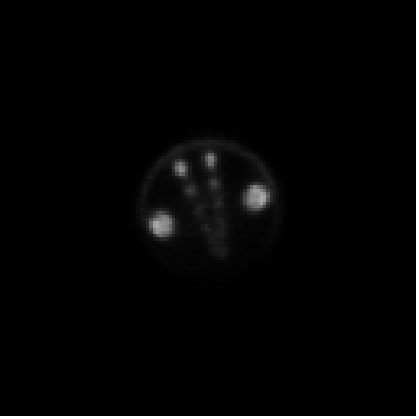
\includegraphics[width=\linewidth]{kuvat/pro_specta_rekonstruktio_proj1_malli3_nRay9.pdf}
        \caption{Sädepohjainen projektiomenetelmä, malli 3, 9 sädettä}
    \end{subfigure}
    \caption{Symbia Pro.specta -laitteella mitatun projektiodatan rekonstruktio neljällä eri projektiomenetelmällä ja laitevalmistajan ohjelmistolla. Kuvissa on esitetty poikkileikkaus kuva-alueen aktiivisuusjakaumasta. Kuvien värikartat ovat skaalattu siten, että kuva-alueen suurin arvo vastaa valkoista väriä ja kuva-alueen pienin arvo mustaa väriä. Kuvan \textbf{(c)} rekonstruktion projektiossa käytettiin 7 sädettä yhtä kollimaattorin reikää kohti. Kuvan \textbf{(e)} rekonstruktiossa säteiden määrä voi olla vain jonkin luonnollisen luvun neliö, josta johtuen rekonstruktioon valittiin 9 sädettä.}
    \label{fig:rekonstruktiot}
\end{figure}

\hyperref[fig:laskenta_aika]{Kuvassa \ref*{fig:laskenta_aika}} on esitetty mallin 3 sadan rekonstruktion keskimääräinen laskenta-aika säteiden lukumäärän funktiona sekä kahden keskihajonnan väli. Kuvaajasta nähdään, että käytetyllä laitteistolla laskenta-aika sekunneissa on likimäärin säteiden lukumäärä kaksinkertaisena. \hyperref[fig:laskenta_aika]{Kuvan \ref*{fig:laskenta_aika}} suoran kulmakerroin riippuu lähinnä laskennassa käytetyn suorittimen tehokkuudesta, iteraatioiden ja osajoukkojen lukumäärästä sekä kuva-alueen ja detektoripaneelin resoluutiosta.

\begin{figure}[H]
    \centering
    \captionsetup{width=.9\linewidth}
    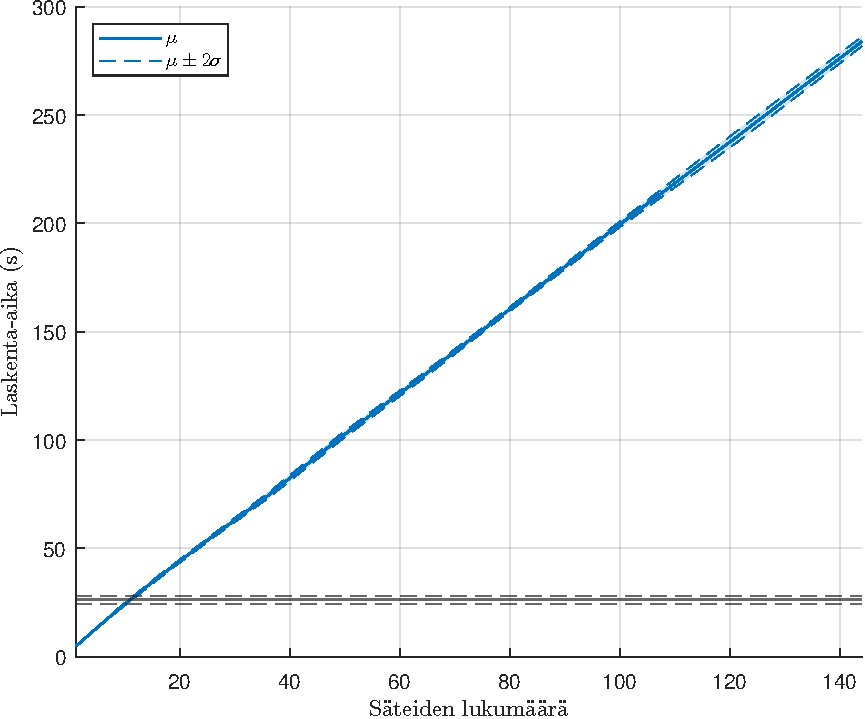
\includegraphics[width=.9\linewidth]{kuvat/laskenta_aika.pdf}
    \caption{Kuvan rekonstruktion laskenta-aika mallin 3 sädepohjaisella projektiolla (sininen väri) ja kuva-alueen rotaatioon perustuvalla projektiolla (harmaa väri). Yhtenäisellä viivalla on piirretty rekonstruktion keskimääräinen laskenta-aika ($N=100$) säteiden lukumäärän funktiona. Katkoviivoilla on havainnollistettu kahden keskihajonnan vaihteluväliä. Laskennassa käytetty suoritin oli Intel i7-10850H.}
    \label{fig:laskenta_aika}
\end{figure}

Mallilla 3 toteutetun rekonstruktion yhtäläisyyttä fantomiin eri säteiden lukumäärällä verrattiin \textit{structural similarity index measure} (SSIM) -mittarilla\cite{wang_image_2004} sekä keskivirheellä (\textit{mean square error}, MSE). SSIM-arvo 1 ja MSE-arvo 0 tarkoittavat, että kuvat ovat täsmälleen samankaltaiset. Vastaavasti pienemmillä SSIM-arvoilla ja suuremmilla MSE-arvoilla kuvissa on enemmän eroavaisuuksia. Vertailun tulokset ovat esitetty \hyperref[fig:vertailu_SSIM]{kuvassa \ref*{fig:vertailu_SSIM}} ja \hyperref[fig:vertailu_MSE]{kuvassa \ref*{fig:vertailu_MSE}}.

\begin{figure}[H]
    \centering
    \captionsetup{width=.9\linewidth}
    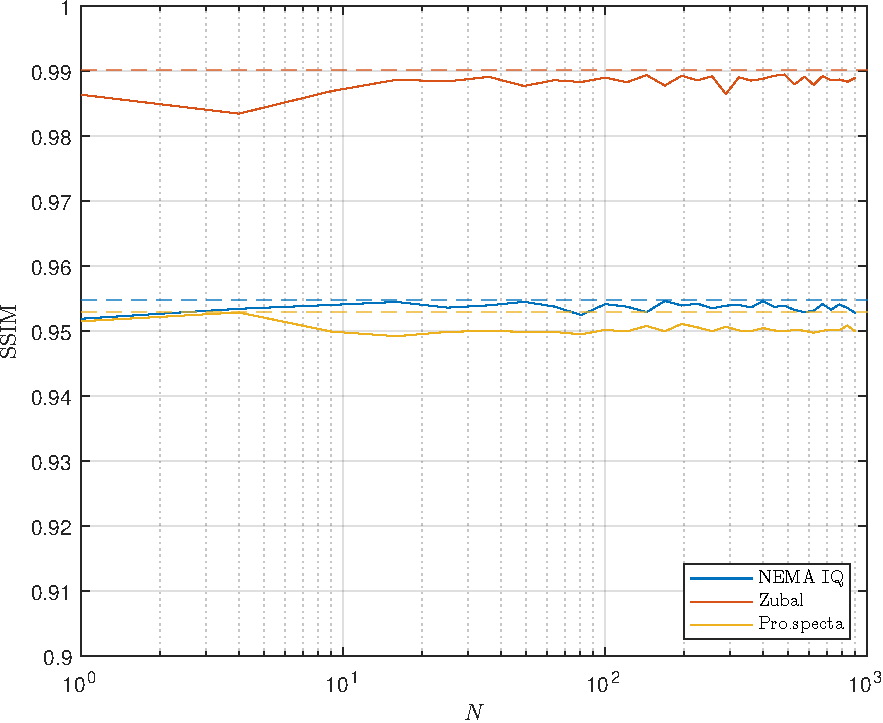
\includegraphics[width=.9\linewidth]{kuvat/vertailu_SSIM.pdf}
    \caption{Simuloidun IQ NEMA -fantomin (sinisellä), simuloidun Zubal-fantomin (punaisella) ja Pro.specta -laitteella mitatun fantomin (keltaisella) SPECT-projektiodatan rekonstruktion vertailu todelliseen aktiivisuusjakaumaan SSIM-mittarilla. Rekonstruktio toteutettiin sädepohjaisella mallilla 3 (yhtenäinen viiva) ja kuva-alueen rotaatioon perustuvalla projektiolla (katkoviiva). Mitatun datan tapauksessa kuvaa todellisesta aktiivisuusjakaumasta ei ollut saatavilla, joten rekonstruktiota verrattiin laitevalmistajan ohjelmistolla tuotettuun rekonstruktioon. Säteiden määrä $N$ on esitetty vaaka-akselilla.}
    \label{fig:vertailu_SSIM}
\end{figure}
\begin{figure}[H]
    \centering
    \captionsetup{width=.9\linewidth}
    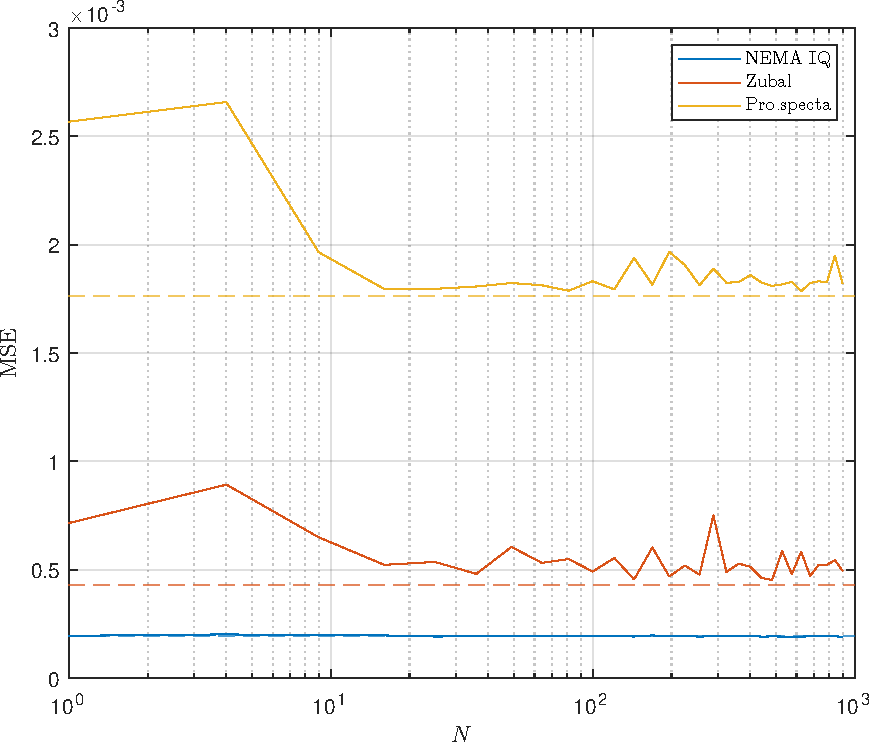
\includegraphics[width=.9\linewidth]{kuvat/vertailu_MSE.pdf}
    \caption{Simuloidun IQ NEMA -fantomin (sinisellä), simuloidun Zubal-fantomin (punaisella) ja Pro.specta -laitteella mitatun fantomin (keltaisella) SPECT-projektiodatan rekonstruktion vertailu todelliseen aktiivisuusjakaumaan keskivirheellä (\textit{mean square error, MSE}). Rekonstruktio toteutettiin sädepohjaisella mallilla 3 (yhtenäinen viiva) ja kuva-alueen rotaatioon perustuvalla projektiolla (katkoviiva). Mitatun datan tapauksessa kuvaa todellisesta aktiivisuusjakaumasta ei ollut saatavilla, joten rekonstruktiota verrattiin laitevalmistajan ohjelmistolla tuotettuun rekonstruktioon.  Säteiden määrä $N$ on esitetty vaaka-akselilla.}
    \label{fig:vertailu_MSE}
\end{figure}

\iffalse
\begin{figure}[H]
    \centering
    \captionsetup{width=.9\linewidth}
    \begin{subfigure}[t]{.4\textwidth}
        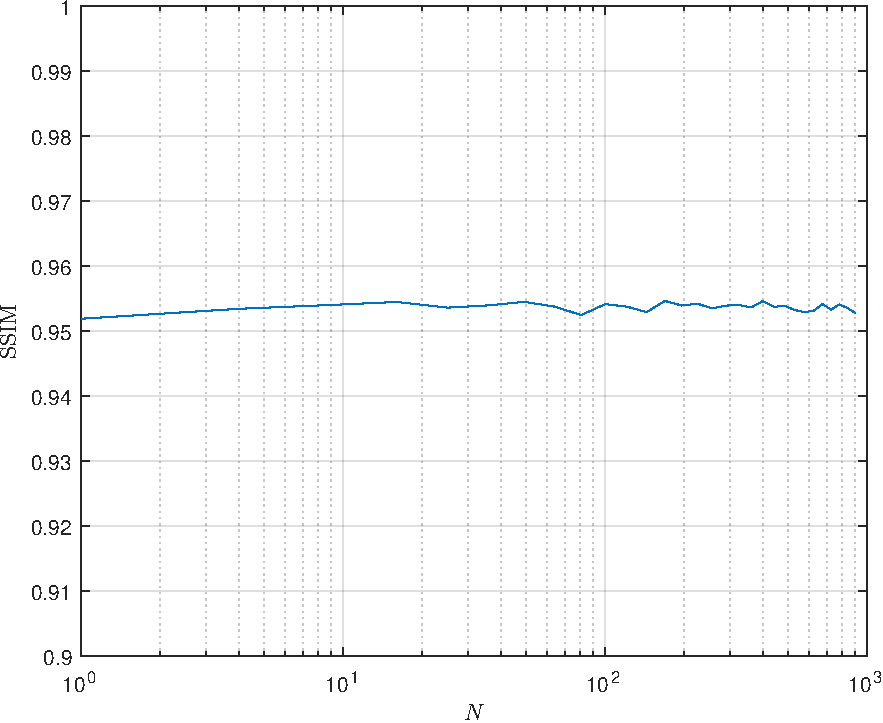
\includegraphics[width=\linewidth]{kuvat/nema_vertailu_SSIM.pdf}
        \caption{IQ NEMA -fantomi}
    \end{subfigure}%
    \hspace{.1\textwidth}%
    \begin{subfigure}[t]{.4\textwidth}
        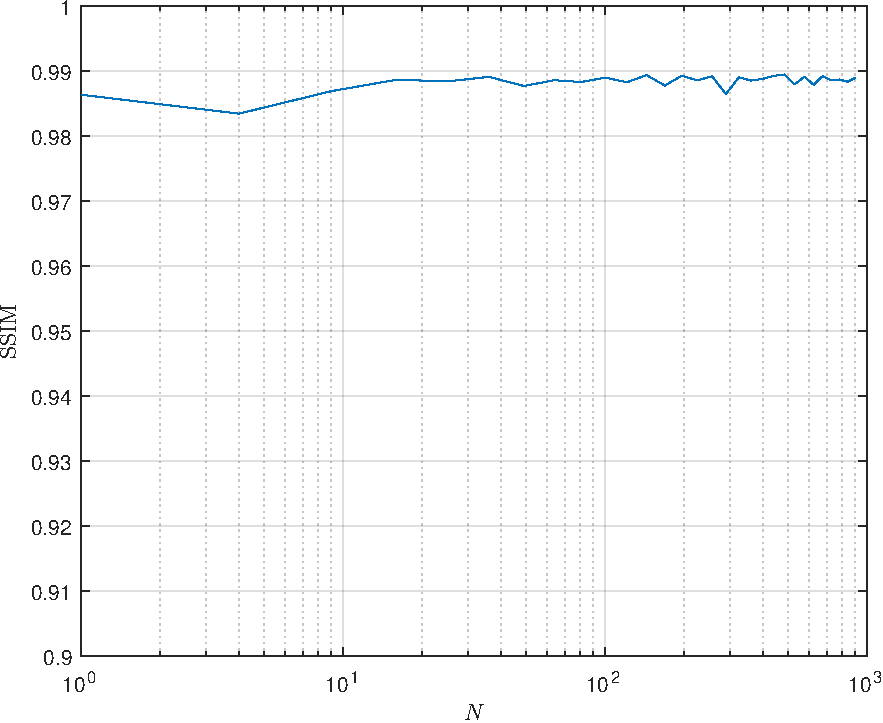
\includegraphics[width=\linewidth]{kuvat/cbf_vertailu_SSIM.pdf}
        \caption{Zubal-fantomi}
    \end{subfigure}%
    \caption{Simuloidun IQ NEMA -fantomin ja Zubal-fantomin SPECT-projektiodatan rekonstruktion vertailu todelliseen aktiivisuusjakaumaan SSIM-mittarilla. Rekonstruktio toteutettiin sädepohjaisella mallilla 3, jossa säteiden määrä on esitetty vaaka-akselilla.}
    \label{fig:vertailu_SSIM}
\end{figure}
\begin{figure}[H]
    \centering
    \captionsetup{width=.9\linewidth}
    \begin{subfigure}[t]{.4\textwidth}
        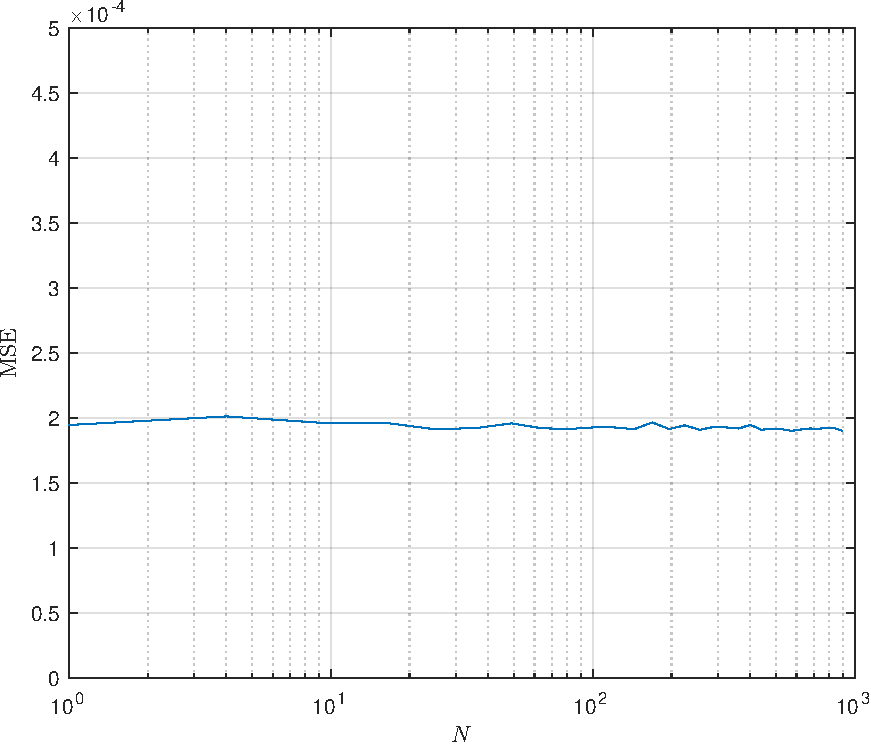
\includegraphics[width=\linewidth]{kuvat/nema_vertailu_MSE.pdf}
        \caption{IQ NEMA -fantomi}
    \end{subfigure}%
    \hspace{.1\textwidth}%
    \begin{subfigure}[t]{.4\textwidth}
        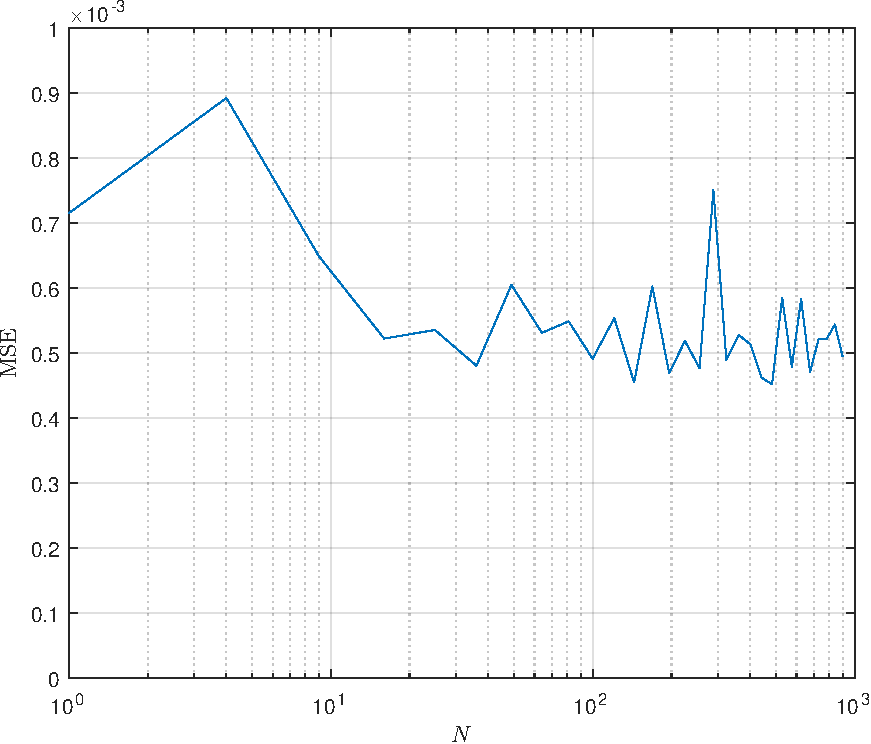
\includegraphics[width=\linewidth]{kuvat/cbf_vertailu_MSE.pdf}
        \caption{Zubal-fantomi}
    \end{subfigure}%
    \caption{Simuloidun IQ NEMA -fantomin ja Zubal-fantomin SPECT-projektiodatan rekonstruktion vertailu todelliseen aktiivisuusjakaumaan keskivirheellä (\textit{mean square error, MSE}). Rekonstruktio toteutettiin sädepohjaisella mallilla 3, jossa säteiden määrä on esitetty vaaka-akselilla.}
    \label{fig:vertailu_MSE}
\end{figure}
\fi

\iffalse
Kuviin \ref{fig:rekonstruktio4}, \ref{fig:rekonstruktio64} ja \ref{fig:rekonstruktio144} on piirretty projektiodatan rekonstruktio 4, 64 ja 144 säteellä. Jokainen rekonstruktioista on selkeä, mutta yksityiskohdat ja muutokset aktiivisuusjakaumassa tarkentuvat säteiden määrän kasvaessa.
\begin{figure}[H]
    \centering
    \captionsetup{width=.9\linewidth}
    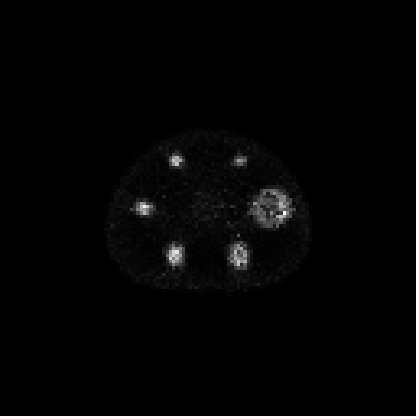
\includegraphics[width=.9\linewidth]{kuvat/rekonstruktio_nRay4.pdf}
    \caption{NEMA-fantomista simuloidun projektiodatan rekonstruktio. Projektioita on 64, tasaisesti joka puolelta kuva-aluetta. Mallissa jokainen detektorin pikseli havaitsee gammafotoneja 4 eri suunnasta.}
    \label{fig:rekonstruktio4}
\end{figure}
\begin{figure}[H]
    \centering
    \captionsetup{width=.9\linewidth}
    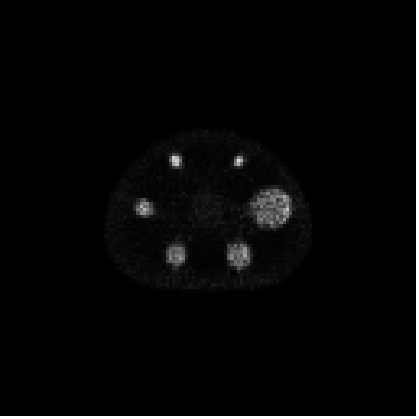
\includegraphics[width=.9\linewidth]{kuvat/rekonstruktio_nRay64.pdf}
    \caption{NEMA-fantomista simuloidun projektiodatan rekonstruktio. Projektioita on 64, tasaisesti joka puolelta kuva-aluetta. Mallissa jokainen detektorin pikseli havaitsee gammafotoneja 64 eri suunnasta.}
    \label{fig:rekonstruktio64}
\end{figure}
\begin{figure}[H]
    \centering
    \captionsetup{width=.9\linewidth}
    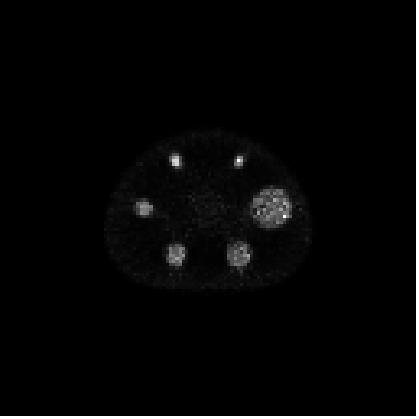
\includegraphics[width=.9\linewidth]{kuvat/rekonstruktio_nRay144.pdf}
    \caption{NEMA-fantomista simuloidun projektiodatan rekonstruktio. Projektioita on 64, tasaisesti joka puolelta kuva-aluetta. Mallissa jokainen detektorin pikseli havaitsee gammafotoneja 144 eri suunnasta.}
    \label{fig:rekonstruktio144}
\end{figure}
\fi